\documentclass[times, 10pt, twocolumn]{article}
\usepackage{latex8}
\usepackage[dvips]{graphicx}
\usepackage[fleqn]{amsmath}
\usepackage{amsthm}
\usepackage{txfonts}
\usepackage{courier}
\usepackage{subfigure}
\usepackage{comment}
\usepackage{url}
\usepackage[square,numbers]{natbib}

\newcommand{\hd}{\emph{H+D}}
\newcommand{\hp}{\emph{Hpin}}
\newcommand{\dm}{\emph{Dmap}}

%-----------------------------------------
% need for camera-ready
%\pagestyle{empty}

%----------------------------------------


\title{Toward GPU-accelerated Traffic Simulation and Its Real-Time Challenge}

\author {
Manato Hirabayashi, Shinpei Kato, Masato Edahiro\\
\textit{Department of Information Engineering}\\
\textit{Nagoya University}\\
\and
Yuki Sugiyama\\
\textit{Department of Complex Systems Science}\\
\textit{Nagoya University}\\
}

\begin{document}

\maketitle

%-----------------------------------------
% need for camera-ready
%\thispagestyle{empty}

\begin{abstract}
 Traffic simulation is a growing domain of computational physics.
 There are many applications in our life and industry that benefit
 from traffic simulation.
 A core challenge of this science research, however, is posed due to
 an unbounded scale of computation.
 In this paper, we explore an advantage of using the graphics processing
 unit (GPU) to support its computation.
 Two schemes are presented to study how to maximize GPU
 performance in the context of traffic simulation.
 Our experimental results show that even the most basic GPU
 implementation based on our schemes accelerates simulation by about
 five times over the original CPU implementation.
 We also demonstrate that additional orders-of-magnitude
 improvements could be achieved by overcoming the current hardware
 limitation.
\end{abstract}

\section{Introduction}

Transportation systems underlie our life and industry, as part of
societal infrastructure.
Traffic flow is particularly a major factor that influences economy.
According to the Japanese government report, economic losses due to
traffic congestion could reach one hundred billion dollars per year in
Japan, through degradation of transport efficiency, energy consumption,
and environmental poisoning.
Albeit a major issue of transportation systems, the mechanism of traffic
congestion is not well-explained in the literature.
What is particularly important is ``phantom jam'', which often happens
on freeways without any accident.
This phantom jam should be avoided by science, given that it is
a physical phenomenon but not one caused by human errors.
However, we have not been aware of scientific and engineering solutions
to such real-world problems yet.

In physics, traffic flow is described by mathematical
models~\cite{Bando1995, Bando1995_2, Kerner1993, Nagel1992}.
While their mathematical expressions are not identical, they are
commonly compute-intensive forms.
For example, traffic simulation based on the Optimal Velocity (OV)
model~\cite{Bando1995, Bando1995_2} computes locations and velocities of
agents every sampling period, solving OV equations. 
Specifically, the location $x_n$ of the $n$th agent is described by the
following equation, where $\Delta x_n = x_{n+1} - x_n$ is a distance to
a preceding agent, $a$ is a sensitivity, and $V()$ is an optimal
velocity function:
\begin{eqnarray}
 \label{eqn:ov}
 \frac{d^2 x_n}{d t^2} = a \left\{V(\Delta x_n) - \frac{d x_n}{d t}\right\}.
\end{eqnarray}

Applying a large number of agents to simulation using the above formula,
it is apparent that computational workload increases exponentially.
In fact, the above formula considers only one dimension, which restricts
applications of simulation to freeway traffic flows, powder flows,
molecular motors, and so on.
Making it multi-dimensional further increases computational workload,
while allowing more complicated simulations, such as traffic networks,
internet packet flows, evacuation routes, and herd formations of
animals, to use similar optimal velocity models.
Given a scale of million agents in the real world, traffic
simulation should be supported by powerful computer systems.

Computational workload is not the only issue of concern.
Deployment of traffic simulation may also require real-time feedback
from the real world, which turns out to be a cyber-physical systems
(CPS) problem indeed.
Real-time traffic simulation is another challenging issue, where
the rate and the preciseness of simulation must be traded to meet the
requirement of a given scenario.
For instance, simulation of emergent evacuation may want very high-rate
computation, even sacrificing preciseness of simulation to some extent.
Unfortunately, none of those challenges has been explored yet, largely
due to a lack of multidisciplinary collaborations between computational
physics and computer science.

This paper explores how to accelerate traffic simulation using the
state-of-the-art parallel computing technology.
In particular, we use the graphics processing unit (GPU), which
integrates hundreds of cores on a chip.
Recent GPUs are becoming more and more suitable for general-purpose
data-parallel applications.
The traffic simulation program used in this paper applies
Equation~\eqref{eqn:ov} to a large number of agents.
The resulting workload is highly data-parallel and compute-intensive,
which can be nicely offloaded on to the GPU.
We also identify the bottleneck in accelerating our traffic simulation
program using the GPU, and provide some insight into its solution.

The rest of this paper is organized as follows.
Section~\ref{sec:assumption} describes the basic assumption and
terminology used in this paper.
Section~\ref{sec:traffic_simulation} explains an overview of
traffic simulation and its literature.
Section~\ref{sec:gpu_implementations} presents our schemes of GPU
implementations for traffic simulation.
Section~\ref{sec:evaluation} evaluates the advantage of using our
schemes, and provides an insight into future work.
Section~\ref{sec:conclusion} concludes this paper.

\section{Assumption and Terminology}
\label{sec:assumption}

We assume the Compute Unified Device Architecture (CUDA) for GPU
programming.
In CUDA, a unit of pieces of code that is launched on the GPU is called
a \textit{kernel}.
The kernel is typically composed of multiple \textit{threads} that
executes the code in parallel.
A unit of threads that are co-scheduled by hardware is called a
\textit{block}, while a collection of blocks for the corresponding
kernel is called a \textit{grid}.  
The maximum number of threads that can be contained by an individual
block is defined by the GPU architecture.

CUDA programs use a set of the application programming interface (API)
functions to control the GPU.
We usually take the following steps to use the GPU: (i) allocate space
to device memory, (ii) copy data to the allocated device memory space,
(iii) launch the program on the GPU, (iv) copy resultant data back to
host memory, and (v) free the allocated device memory space. 

Our computing platform is composed of a single CPU and GPU.
The traffic simulation program is a single process from the CPU point of
view.
Hence, kernels are launched from the CPU sequentially, while each kernel
is executed by parallelized threads on the GPU.

While we are intensively interested in CUDA and GPUs, the notion of
accelerating traffic simulation presented in this paper is widely
applicable to heterogeneous architectures, where CPUs and 
accelerators co-exist to complement each other. 
GPUs are currently the most well-recognized forms of accelerators, but
emerging alternatives include the Intel Many Integrated Core (MIC) and
AMD Fusion architectures.
However, their programming models are almost identical in that a master
thread running on the CPU manages the program flow, while parallelized
threads are offloaded on to accelerators to boost computing performance.
CUDA, OpenCL, HMPP, and AMP are all such programming languages that
support heterogeneous architectures under this concept.

\section{Traffic Simulation}
\label{sec:traffic_simulation}

The motivation to study traffic flow is to understand the property of
traffic flow, mainly why traffic congestion occurs.
The study of traffic flow has a long history, and many engineering and
physical models exist.
This paper is particularly focused on the OV model~\cite{Bando1995,
Bando1995_2}.
In this model, a driver is supposed to maintain an optimal velocity that
depends on the driver's headway.
Its motion is given by Equation~\eqref{eqn:ov}.
The optimal velocity function introduced in this equation is represented
by the relationship between the driver's headway and velocity.

The OV model has a simple form with a single parameter of sensitivity
$a$.
This simplicity allows us to understand the mechanisms of phenomena, and
also predict the results of experiments.
The disadvantage of this model, on the other hand, is a little allowance
for control systems to turn up the parameter.
There is indeed a need for collaborations between the research domains
of engineering and physics.
To begin with, however, we restrict our attention to the OV model.
More details are found in~\cite{Bando1995, Bando1995_2}.

The traffic simulation program based on the OV model is straightforward,
as the model itself has a simple form.
In this paper, we abstract its algorithm by the following stages:

\begin{enumerate}
 \item Initialize the time $t$, and set the initial values of $x_n(t)$
       (also $y_n(t)$ and $z_n(t)$, if necessary for multidimensional
       versions).
 \item Increase the time $t$ by the sampling period $\Delta t$.
 \item Compute the location $x_n(t)$ (also $y_n(t)$ and $z_n(t)$, if
       necessary for multidimensional versions), and the velocity
       $v_x(t)$ at time $t$ for each agent $A_n$, using the OV model.
 \item Go back to Step 2, if the simulation time is expired.
 \item Exit the program.
\end{enumerate}

The computational workload in Step 3 exploits a lot of loop executions
to derive locations and velocities of agents.
This is the most compute-intensive part of the algorithm.
The primary goal of this paper is to find out the parallelism of this
workload that can be applied to the GPU.
By nature, traffic simulation based on the OV model is very scalable in
terms of performance with respect to the number of agents.
The location and velocity of each agent depends on only those of
neighbors.
It is worth exploring a breakthrough of this research domain by
coordinating computational physics and computer science technology.

\section{GPU Implementation}
\label{sec:gpu_implementations}

The primary contribution of this paper is to identify the fundamental
schemes of GPU implementations for traffic simulation.
It is very important to understand that GPU performance is dominated by
the program design.
We first reason about the motivation of our schemes.

GPU-accelerated programs are typically divided into two pieces of code.
The CPU code plays a role of a master thread that controls the program
flow.
The GPU code, on the other hand, spawns a bunch of worker threads to
execute compute-intensive parts of the program in parallel, thus
accelerating the overall program.
What is often argued in performance optimization is how to parallelize
the compute-intensive parts into threads.
This is actually the well-studied problem in the literature.
What is not really understood yet is when to offload the program on to
the GPU.
This paper explores two schemes that use the GPU at different timings to
see how GPU performance is affected.

\subsection{Sample-in-CPU Scheme}
\label{sec:sample-in-cpu}

We first implement such a scheme that uses the GPU \textit{only if
necessary}.
In other words, the program is offloaded on to the GPU, only when
computations of locations and velocities of agents are accelerated by
parallelization.
The CPU bridges across sampling periods to manage simulation.
In this scheme, the control flow of simulation is always returned to the
CPU at the end of each sampling period.
Such a synchronized approach makes the programmer easy to
obtain intermediate results of simulation, whereas the overhead imposed
on moving back and forth between the CPU and the GPU must be
compromised.

\begin{figure}[t]
\centering
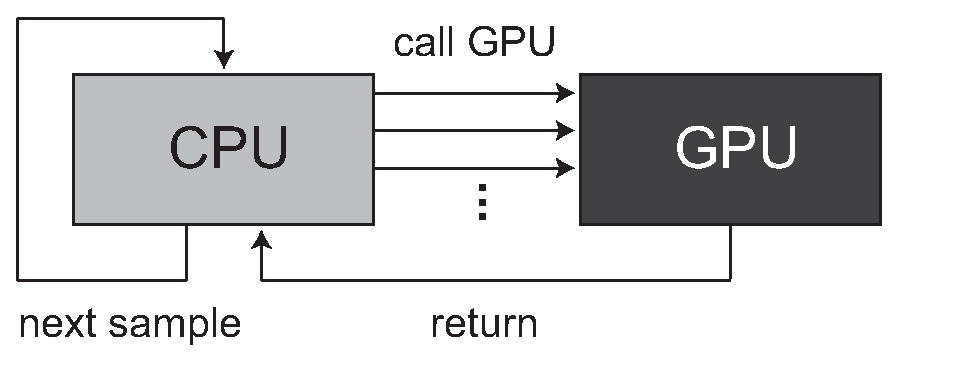
\includegraphics[width=0.4\textwidth]{eps/sample-in-cpu.eps}
\caption{Block diagram of the Sample-in-CPU scheme.}
\label{fig:sample-in-cpu}
\end{figure}

Figure~\ref{fig:sample-in-cpu} shows a brief overview of the
Sample-in-CPU scheme.
This scheme also has several alternatives depending on how many kernels
need to be launched on the GPU in each period. 
Suppose that we want to offload $n$ pieces of \textit{for} loops on to
the GPU.
We may return to the CPU $n$ times in total, that is, return every time
one \textit{for} loop breaks, or otherwise we may just return once when
all the $n$ \textit{for} loops end.
This is a design decision, and is also dependent on the GPU architecture
and the parallelization structure.
In general, parallelized threads need to be synchronized when moving
across basic blocks.
Specifically, when moving to the next \textit{for} loop executed in
parallel, all the threads relevant to this parallel computing procedure
must synchronize with each other.
However, the maximum number of threads that can be synchronized on the
GPU is often limited.
As of 2012, for example, NVIDIA's GPU architectures limit the number of
such threads to 1024 or less~\cite{NVIDIA_Kepler}.
Our implementation therefore forces the program to return to the CPU
every time one \textit{for} loop breaks.
Note that this is not a conceptual limitation of GPU computing, but is a
current limitation of hardware.
We believe that this limitation would be removed or mitigated in
next-generation GPU architectures.

\subsection{Sample-in-GPU Scheme}
\label{sec:sample-in-gpu}

\begin{figure}[t]
\centering
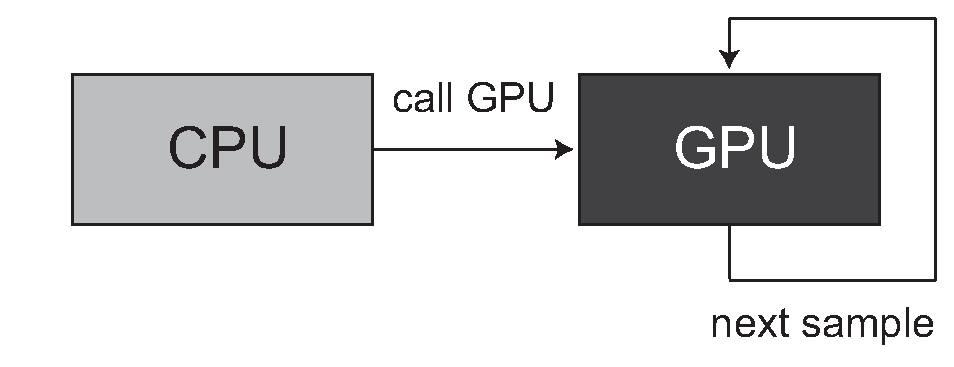
\includegraphics[width=0.4\textwidth]{eps/sample-in-gpu.eps}
\caption{Block diagram of the Sample-in-GPU scheme.}
\label{fig:sample-in-gpu}
\end{figure}

We next implement such a scheme that uses the GPU \textit{all the time},
even to control simulation.
There is one big kernel running on the GPU, which is launched only once
at the beginning.
After offloading the program on to the GPU, the CPU is going to wait for
the completion of simulation.
This scheme is almost optimized in performance, since there is little
overhead in communication between the CPU and the GPU.
The downside of this scheme is that the CPU and the GPU are not
synchronized.
The progress of simulation is not visible from the CPU, unless the
program implements a specific interface to allow the CPU to access
intermediate results of simulation running on the GPU.
In our implementation, we consider providing a framework that the CPU
downloads data from the GPU asynchronously without awareness of
simulation, when the user requests intermediate results.
This asynchronous data access may affect the performance of simulation,
though in reality this access would not happen more than once in a
sampling period.

Figure~\ref{fig:sample-in-gpu} shows a block diagram of the
Sample-in-GPU scheme.
The procedure is very simple.
The most portion of code of simulation is executed on the GPU.
Given that the single-thread performance of recent GPUs is getting more
reliable, this approach is pretty reasonable.
As mentioned in Section~\ref{sec:sample-in-cpu}, however, the current
limitation of the GPU architecture prevents us from synchronizing among
blocks at a scale of thousands threads.
Therefore, this scheme is speculative in a sense that it does not work today
but may appear in the future.

This paper provides some degree of insights into how this scheme is
effective.
We implement this scheme with the current GPU architecture under the
assumption that global synchronization among blocks works.
There is also another possible approach for this scheme that we limit
the number of threads to what is supported by the GPU architecture.
This alternative implementation, however, is left open for future work.

\section{Evaluation}
\label{sec:evaluation}

We evaluate the performance of our GPU-accelerated traffic simulation
programs, using an NVIDIA GeForce GTX 560 Ti graphics card.
This is a middle-end graphics card based on the Fermi
architecture~\cite{NVIDIA_Fermi}, integrating 394 compute cores on a chip.
The programs used in this evaluation are written in CUDA, and are
compiled by the NVIDIA CUDA Compiler (NVCC) v4.2 suite~\cite{CUDA42}.

We focus on the one-dimensional OV model~\cite{Bando1995, Bando1995_2},
which can be applied to freeways simulation.
The original program~\cite{OV_Program} of this simulation is written in
C, without any parallelization.
We use the same simulation parameters as the original default setup,
while increasing the number of agents (cars) to see how simulation
performance varies. 
The evaluation is conducted by comparing our GPU implementations with
the original CPU implementation.

\subsection{Performance Benefit}

\begin{figure}[t]
\centering
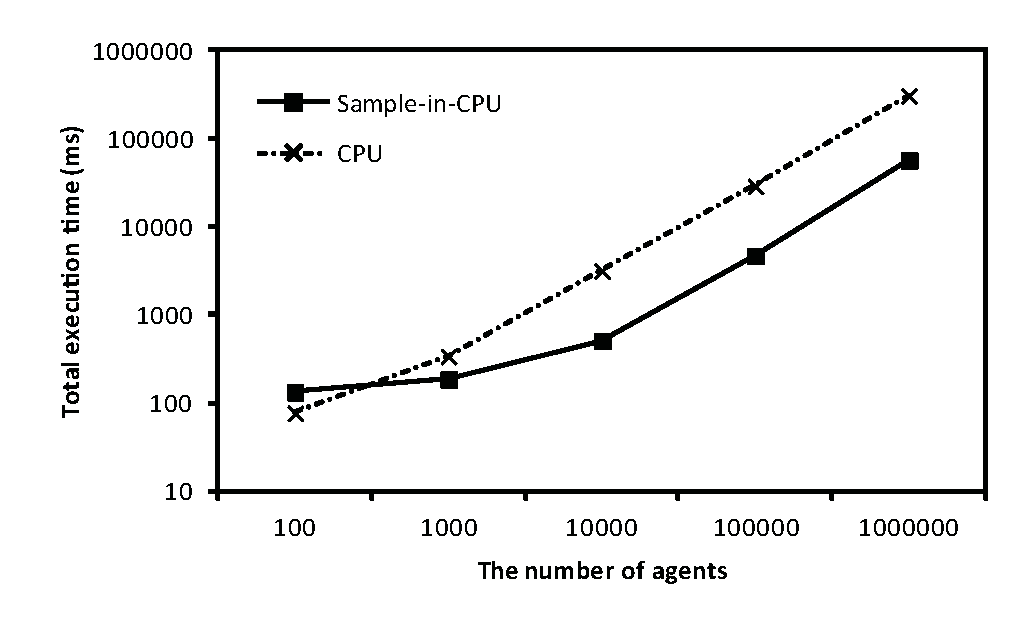
\includegraphics[width=0.5\textwidth]{eps/eval_accel.eps}
\caption{Performance benefit of the GPU.}
\label{fig:eval_benefit}
\end{figure}

Figure~\ref{fig:eval_benefit} demonstrates the performance benefit of
the GPU under the current hardware limitation.
The Sample-in-CPU scheme herein exploits synchronization between the CPU
and the GPU after every \textit{for} loop to overcome the limitation that
CUDA threads cannot synchronize beyond blocks.
Despite of this restricted implementation, our GPU implementation
outperforms the original CPU implementation by about five times in
simulation time, when the number of agents exceeds a scale of 1000.
This evinces an affinity of the GPU and parallel computing for traffic
simulation.
It is also interesting to see that the CPU implementation has a better
performance for a small number of agents.
Thus, the overhead of communication between the CPU and the GPU has
non-trivial impact if the achievable parallelism is not sufficient.
Another notable observation is that the difference in performance of the
CPU and the GPU implementations is saturated when the number of agents
reaches 1000.
This saturation implies the hardware potential of the NVIDIA GeForce GTX
560 Ti graphics card used in this evaluation.
Using high-end graphics cards, the difference in performance may not be
saturated at the same scale.

\subsection{Impact of Hardware Limitation}

\begin{figure}[t]
\centering
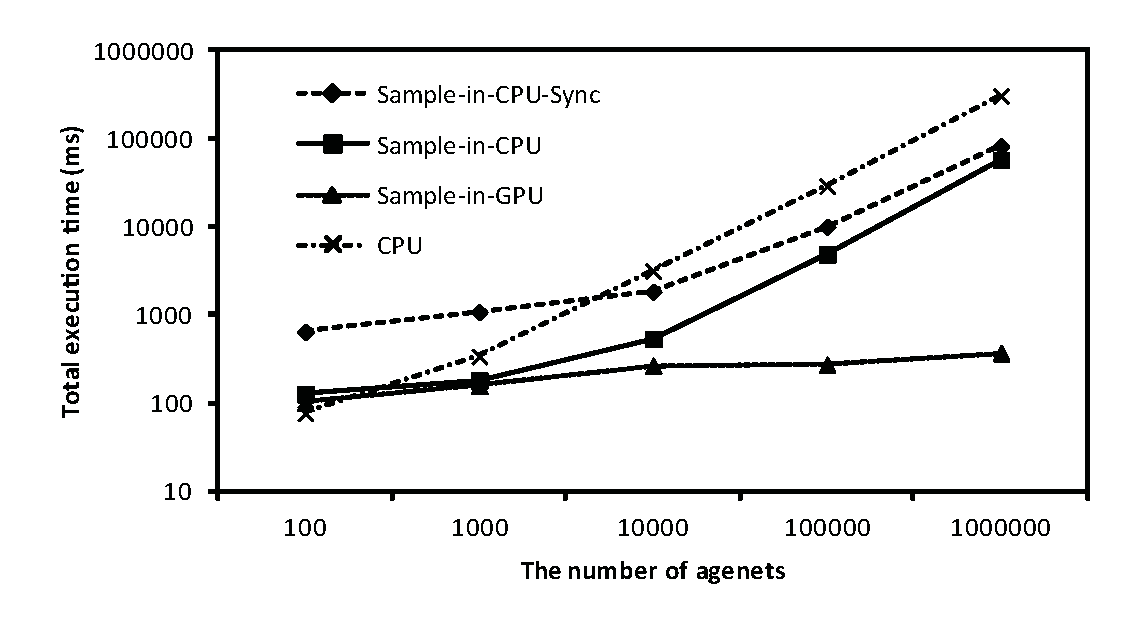
\includegraphics[width=0.5\textwidth]{eps/eval_nosync.eps}
\caption{Impact of the hardware limitation.}
\label{fig:eval_nosync}
\end{figure}

Figure~\ref{fig:eval_nosync} demonstrates the impact of the current
hardware limitation that CUDA threads cannot synchronize beyond blocks.
In this experiment, we observe ``what would happen if this hardware
limitation is removed?'', compromising the preciseness of simulation
results.
Namely, we use the current CUDA synchronization function to synchronize
threads running in different blocks, even though it does not work as
expected.
All the GPU implementations of the plotted schemes use this assumption.
Therefore, the Sample-in-CPU scheme is now different from what we have
evaluated in Figure~\ref{fig:eval_benefit}, since there is no need
anymore to return to the CPU every time one \textit{for} loop breaks.
We instead put a synchronization function between \textit{for} loops on
the GPU.
The Sample-in-CPU-Sync scheme is an alternative version of the
Sample-in-CPU scheme in that we download intermediate results from the
GPU to the CPU at the end of each sampling period.
The Sample-in-GPU scheme is what is presented in
Section~\ref{sec:sample-in-gpu}.

It is very notable that the Sample-in-GPU scheme improves the simulation
time by a factor of 1000 as compared to the original CPU implementation.
This result encourage support for thread synchronization among blocks in
CUDA programming.
There are also several interesting observations obtained in this
experiment.
Comparing the Sample-in-CPU and the Sample-in-CPU-Sync schemes, it turns
out that the cost of downloading intermediate results from the GPU to
the CPU is becoming trivial as the scale of simulation increases.
Hence, a common argument of ``host-device data communication in GPU
programming is expensive'' does not apply to large-scale traffic
simulation.
Another issue of concern often discussed in GPU programming is that
a single-thread performance of GPUs is weak as compared to that of CPUs.
This is true in general, but our experimental result shows that the
performance loss caused by pushing most pieces of code into the GPU in
the Sample-in-GPU scheme is not significant even for a small number of
agents.
This observation leads to some conclusion that the Sample-in-GPU scheme
would be the best choice for any scale of traffic simulation.

\subsection{Practical Concern}

\begin{figure}[t]
\centering
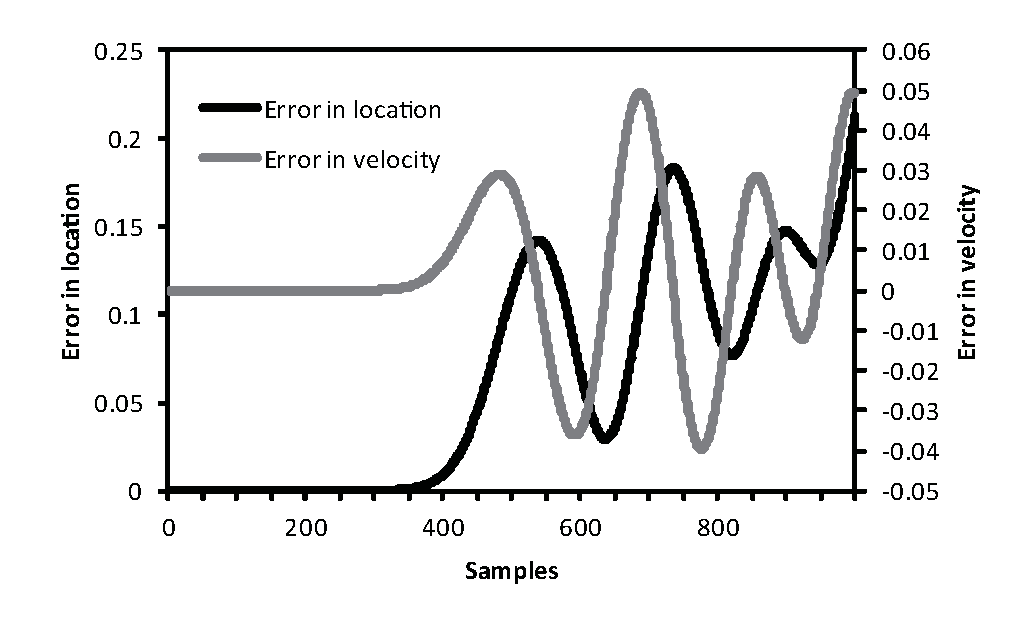
\includegraphics[width=0.5\textwidth]{eps/eval_error.eps}
\caption{Error in location and velocity due to imprecise synchronization.}
\label{fig:eval_error}
\end{figure}

We finally examine the impact of misbehavior of thread synchronization
in our GPU implementations.
The simulation results produced by our GPU implementations are not
precise except for those of the Sample-in-CPU scheme presented in
Figure~\ref{fig:eval_benefit}, due to our optimistic use of thread
synchronization on the GPU.
We need to wait for new GPU architectures removing the limitation of
thread synchronization in order to make them precise.
Practically speaking, however, imprecise results of simulation are still
valuable and meaningful as far as they are limited to an acceptable
range of errors for traffic flow.

Figure~\ref{fig:eval_error} demonstrates the error percentage of
location and velocity between the simulation results produced by the
original CPU and the imprecise Sample-in-GPU implementations.
Since this is one-dimensional OV simulation, there are only forward or
backward in location, and high or low in velocity.
Under this constraint, the error in location is very trivial.
This is because the characteristic of traffic flow is well captured,
even though the simulated locations and velocities have some error in
their individual values.
A degree of the error in velocity is slightly high as compared to that
in location.
This means that velocity is more sensitive to imprecise results than
location.
However, the maximum error in velocity observed in our experiment is at
most 5\%.
Suppose that the average driving speed is 50mph.
The simulated speed in our imprecise implementation would still be
within a range of 47.5 to 52.5mph.
Intuitively, this scale of error is acceptable in practice.
We plan to further investigate if the same argument can be applied to a
more variety of parameter setups and multidimensional OV simulation
programs.

\subsection{Discussion}
\label{sec:discussion}

According to the experimental results, it is highly desired to use the
Sample-in-GPU scheme, if available.
It provides an orders-of-magnitude improvement in simulation time.
The downside of this scheme at the moment is a lack of functionality in
thread synchronization due to the current hardware limitation.
Simulation results are never precise unless thread synchronization
operates correctly.
Although we have demonstrated that the error in simulation results
caused by a lack of thread synchronization is acceptable in our
experimental setup, the range of error is never bounded as depicted in
Figure~\ref{fig:eval_error}.
Hence, the availability of this scheme depends highly on practical
setups.

We consider that the problem of this scheme may be relevant to the
Imprecise Computation model~\cite{Lin1987}.
The Sample-in-CPU scheme is precise-but-slow, while the Sample-in-GPU
scheme is imprecise-but-fast.
If we are allowed to employ multiple GPUs in the system, we may run the
two types of simulation programs on different GPUs concurrently.
At some point of time $t$, the simulation result produced by the
Sample-in-GPU scheme represents a scenario way ahead of that produced by
the Sample-in-CPU scheme; the question is how precise it is.
Figure~\ref{fig:eval_error} demonstrates that the error in the
simulation result produced by the Sample-in-GPU scheme is getting larger
as time goes by.
If we can find such a time duration that causes the value of error to
fall out the acceptable range for practical use, we define this time
duration to be $\Delta t$.
Suppose that the two simulation programs based on the Sample-in-GPU and
the Sample-in-CPU schemes, respectively, are running concurrently.
At every interval of time $\Delta t$, we reset the simulation result
produced by the Sample-in-GPU scheme, and input the latest precise
simulation result produced by the Sample-in-CPU scheme during the same
interval.
By this means, the value of error in the simulation result produced by
the Sample-in-GPU scheme never falls out the acceptable range, while we
still benefit from its simulation speed within an internal of time
$\Delta t$.
The value of $\Delta t$ can be determined dynamically based on the
Imprecise Computation model.

So far we have studied a single process of traffic flow.
In reality, however, there are multiple processes of traffic flow.
Real-time feedback from the real road conditions may also be
additionally required to deploy traffic simulation.
All these pieces of simulation must meet the quality-of-service (QoS)
requirement for users.
Imagine how many potential users exist in the real-world transportation
system.
We are facing a core challenge of next-generation real-time systems.

We have developed basic solutions to use the GPU in real-time
systems~\cite{Kato2011_3, Kato2011_2, Kato2011_1, Kato2012}.
Resource management with scheduling, synchronization, and memory
management of GPU applications has been addressed in our previous
work.
We believe that a grander vision of GPU-accelerated traffic
simulation will need an integration of cutting-edge real-time systems
technology and computational physics.


\section{Conclusion}
\label{sec:conclusion}

In this paper, we have presented GPU-accelerated traffic simulation
based on the OV model.
The current hardware limitation of the GPU architecture caps
improvements in performance to a factor of ten or less, as compared to
the original CPU implementation.
However, we demonstrated that additional orders-of-magnitude
improvements could be achieved by removing that limitation.
We also discussed a conceivable solution to cope with that limitation,
using a concept of the Imprecise Computation model.

In future work, we extend our scheme to multidimensional OV models.
This extension allows our research to be applied to a broader range of
problems beyond freeways traffic simulation.
We also plan to consider a specific approach to the integration of the
Imprecise Computation model into our scheme in order to facilitate
deployment of traffic simulation in the real world.
Another interesting direction in this line of work is to coordinate with
engineering-based simulation such as AutoMatrix~\cite{Mangharam2011}.

\bibliographystyle{plain}
{\footnotesize
\bibliography{references}
}

\end{document}
